% TODO: Kapitel unterkapitel

\chapter{Zynq}
Der Zynq-7000 ist ein SoC (System on Chip), das einen 667 MHz Dual-Core ARM Cortex-A9 Prozessor und eine programmierbare Logik enthält, die einem Artix-7 FPGA entspricht.
Der Prozessor und dessen Peripherie befindet sich im \textit{Processing System} oder kurz PS.
Der FPGA-Teil des Zynq wird oft PL oder \textit{Programmable Logic} genannt.
Über den internen AMBA-Bus kann der Prozessor und auch die PL auf die Peripherie, wie z.B. SPI, GPIO, Ethernet oder auch DDR3, zugreifen.
Das Block Diagramm in der Abbildung \ref{fig:BlockDiagrammZynq} gibt einen guten Überblick über das ganze SoC.
Das restliche Kapitel beschreibt relevante Komponente und Eigenarten des Zynq.

\begin{figure}[htbp]
	\centering
		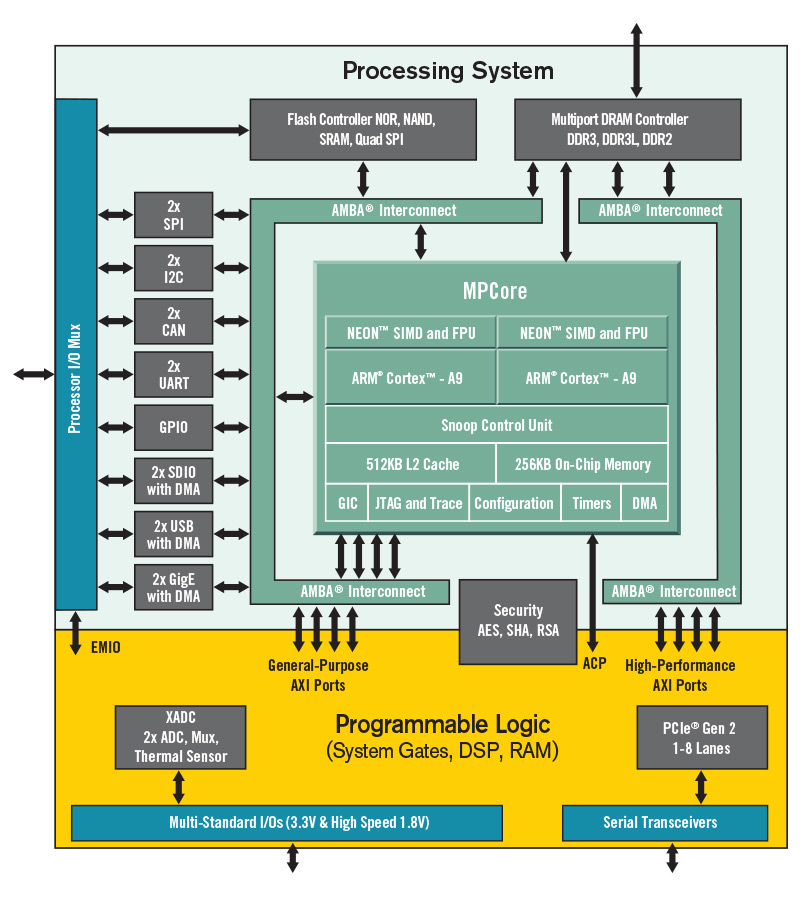
\includegraphics[width=10cm,height=\textheight,keepaspectratio]{images/zynqBlockDiagram.png}
	\caption[Block Diagramm Zynq\-7000]{Block Diagramm Zynq\-7000\footnotemark}
	\label{fig:BlockDiagrammZynq}
\end{figure}
\footnotetext{https://www.xilinx.com/products/silicon-devices/soc/zynq-7000.html}


\section{MIO und EMIO}
MIOs sind \textit{Multiplexed Input Output Pins}, welche direkt vom Prozessor angesprochen werden können, ohne dass die PL programmiert werden muss.
Die EMIOs sind \textit{\textbf{Extended} Multiplexed Input Output Pins}, welche nur über die PL angesprochen werden können.
Aus diesem Grund können die EMIOs nur verwendet werden, wenn die PL entsprechend programmiert wurde.
Diese Arbeit beschränkt sich nur auf die MIOs und das PS.
Im TRM\footnote{Technical Reference Manual} des Zynq\cite{bib:ZynqTechnicalReferenceManual} im Kapitel \textit{''2.5.4 MIO-at-a-Glance Table''} ist eine sehr gute Übersicht über alle möglichen Funktionen der MIOs gegeben.

% TODO MIO config des zybos

\section{Standard Zybo Workflow}
Im \textit{Getting Started with Zynq\footnote{https://reference.digilentinc.com/learn/programmable-logic/tutorials/zybo-getting-started-with-zynq/start?redirect=1}} Tutorial von Digilent ist beschrieben, wie man ein einfaches Design für die PL und ein einfaches Programm für das PS erstellt.
Das Tutorial deckt den ganzen Workflow ab.
Dabei werden, z.B. für LED1, LED2 und LED3, auch die EMIOs verwendet.
In Schritt 1 bis 7 wird mit Vivado das Design für die PL erstellt und exportiert.

\textbf{Hinweis1:} Die Zybo Toolchain benötigt den standard USB-Treiber. Im Kapitel \ref{kapitel:usbTreiber} ist beschrieben, wie der standard USB-Treiber wieder installiert werden kann.

\textbf{Hinweis2:} Vivado und die Xilinx SDK müssen für dieses Tutorial installiert sein.

Ab Schritt 8 wird beschrieben, wie im XSDK (\textit{Xilinx Standard Development Kit}) ein einfaches ''Hello World'' Programm in C für den Prozessor geschrieben werden kann.
% Das XSDK ist Eclipse mit einem Xylinx Plug-In.

Das XSDK verwendet im Hintergrund das XSCT\footnote{https://www.xilinx.com/html\_docs/xilinx2018\_1/SDK\_Doc/xsct/intro/xsct\_introduction.html} (\textit{Xilinx Software Command-Line Tool}).
Das XSDK kann interaktiv, oder mit Scripts verwendet werden.
% Die Scriptsprache basiert, wie auch Jim-TCL, auf der Sprache TCL.
Wie Jim-TCL basiert auch die verwendete Scriptsprache auf der Sprache TCL.
Wird das ''Hello World'' Programm im XSDK gestartet, erscheint im \textit{SDK Log} Fenster ein detailliertes Log des ausgeführten Scripts.
In diesem Log kann nachvollzogen werden, was das Script beim Download und Start des Programms alles ausgeführt hat.

% TODO was auch immer
Im Anhang \ref{anhang:SDKLog} ist eine Kopie eines solchen Logs zu finden.
% TODO: langesWort
\textit{D:/Vivado/01\_gettingStarted/01\_gettingStarted.sdk/.sdk/launch\_scripts/xilinx\_c-c++\_application\_(system\_debugger)/system\_debugger\_using\_debug\_01\_gettingstarted\_applicationproject.elf\_on\_local.tcl}
% \textit{D:/Vivado\01\_gettingStarted\01\_gettingStarted.sdk\.sdk\launch\_scripts\xilinx\_c-c++\_application\_(system\_debugger)\system\_debugger\_using\_debug\_01\_gettingstarted\_applicationproject.elf\_on\_local.tcl}

Das Script \textit{ps7\_init.tcl} definiert unter anderem die fünf Initialisierungs-Methoden:
\begin{itemize}
%\begin{itemize}
\item \textit{ps7\_mio\_init\_data\_3\_0}
\item \textit{ps7\_pll\_init\_data\_3\_0}
\item \textit{ps7\_clock\_init\_data\_3\_0} 
\item \textit{ps7\_ddr\_init\_data\_3\_0}
\item \textit{ps7\_peripherals\_init\_data\_3\_0}
\end{itemize}
Die Initialisierungs-Methoden werden in der Methode \textit{ps7\_init} aufgerufen.
\textit{ps7\_init} wiederum wird in Zeile 8 des \textit{...elf\_on\_local.tcl} Scripts aufgerufen, welches beim Start des ''Hello World'' Programms im XSDK ausgeführt wird.
In Zeile 9 vom \textit{...elf\_on\_local.tcl} wird auch die Methode \textit{ps7\_post\_config} von \textit{ps7\_init.tcl} aufgerufen, welche im Anschluss \textit{ps7\_post\_config\_3\_0} aufruft.

Alle Konfigurationsregister sind im Anhang B vom \textit{Zynq TRM}\cite{bib:ZynqTechnicalReferenceManual} beschrieben.
Bevor die Register aber verändert werden können, müssen sie \textit{''unlocked''} werden, in dem der Wert \textit{0x0000DF0D} in die Adresse \textit{0xF8000008} geschrieben wird.


\subsection{Grundlegende Methoden}
Alle Methoden des \textit{ps7\_init.tcl}-Scripts sind auf den folgenden vier Grundbefehlen aufgebaut:\\
\textbf{mwr -force <address> <value>: }\\
Schreibt den Wert <value> in die Adresse <address>.

\textbf{mask\_write <address> <mask> <value>: }\\
Schreibt die Bits der Maske <mask> von <value> in die Addresse <address>.

\textbf{mask\_poll <address> <mask>:  }\\
Wartet, bis die maskierten Bits <mask> des Speicherinhalts von der Speicheradresse <address> gleich 0 sind.

\textbf{mask\_dellay <address> <value>:}\\
Wartet <value> Millisekunden.

% TODO silikon version überprüfen ps7_init.tcl.745


\subsection{Initialisierungsmethoden}
Im Folgenden werden alle Methoden beschrieben, welche zur Initialisierung des Zynq auf dem Zybo verwendet werden.

\textbf{ps7\_mio\_init\_data\_3\_0:}\\
Diese Methode initialisiert die MIOs.
Der Multiplexer für die IO Pins wird konfiguriert.
Dadurch wird definiert, welcher Pin von welcher Peripherie, wie UART und auch RAM, verwendet wird.
Zusätzlich werden auch, falls vorhanden, folgende elektrischen Charakteristiken definiert:
\begin{itemize}
\item \textbf{Pullup:} Pullup Widerstand aktivieren / deaktivieren.
\item \textbf{IO\_Type:} Buffer Type: LVCMOS 1.8V, LVCMOS 2.5V, LVCMOS 3.3V,  oder HSTL.
\item \textbf{Speed:} Slow oder fast CMOS edge.
\item \textbf{Tristate:} Enalbe / disable Tristate.
\end{itemize} 


\textbf{ps7\_pll\_init\_data\_3\_0}\\
Initialisiert die drei PLLs\footnote{Phase Locked Loop} ARM, DDR und IO.
Bei jeder PLL-Initialisierung wird darauf gewartet, bis der PLL betriebsbereit (locked) ist.
Die Dauer dieser Wartezeit ist unbekannt.

\textbf{ps7\_clock\_init\_data\_3\_0}\\
Konfiguriert diverse Clocks, die im Prozessor gebraucht werden.

\textbf{ps7\_ddr\_init\_data\_3\_0}\\
Konfiguriert den DDR Bus.
Für die Konfiguration werden insgesamt 79 verschiedene Register geschrieben und die DCI (\textit{Digital Controlled Impedance}) kalibriert.

\textbf{ps7\_peripherals\_init\_data\_3\_0}\\
Konfiguriert folgende Peripherien:
\begin{itemize}
\item UART1
\item QSPI (für Flash Speicher auf Zybo)
\item POR timer
\item High-Low-Wait(1msec)-High Sequenz für MIO46 (USB-OTG Ping)
\end{itemize}  




Die oben genannten Initialisierungsfunktionen werden vom Xilinx Debugger jedesmal ausgeführt, wenn die Applikation im XSDK mit \textit{''Launch on Hardware (System Debuger)''} gestartet wird.
Es ist aber auch möglich, die Initialisierung direkt mit der C-Applikation und nicht mit dem Debugger durchzuführen.
Wird die Initialisierung in der Applikation durchgeführt, und die Applikation auf dem Flash Speicher des Zynq gespeichert, dann Initialisiert sich der Zynq bei jedem Start selber.
Im Beispielprogramm \textit{''helloworld.c''} ist die Methode \textit{''init\_platform()''} enthalten, welche in \textit{''platform.c''} deklariert ist.
Standardmässig ist die darin enthaltene Methode \textit{''ps7\_init()''} aber auskommentiert.
\textit{''platform.c''} befindet sich im \textit{''design\_wrapper\_hw\_platform''}, welcher in Vivado erzeugt wurde.
Vergleicht man \textit{''ps7\_init()''} mit \textit{ps7\_init.tcl}, dann sieht man schnell, dass das Script und auch die C-Methode genau die gleichen Register schreiben und lesen.

\textit{''psu\_init()''} ist für ein \textit{''Zynq UltraScale+™ MPSoC''} Chip, welcher auf dem Zybo nicht verwendet wird.


\textit{helloworld.c:}
\lstset{language=c}
\begin{lstlisting}[frame=single]
...
#include "platform.h"
..
int main ()
{
...
init_platform();

while(1){
...
\end{lstlisting}



\textit{platform.c:}
\lstset{language=c}
\begin{lstlisting}[frame=single]
...
/*#include "ps7_init.h"*/
/*#include "psu_init.h"*/
...
void
init_platform()
{
    /*
     * If you want to run this example outside of SDK,
     * uncomment one of the following two lines and also #include "ps7_init.h"
     * or #include "ps7_init.h" at the top, depending on the target.
     * Make sure that the ps7/psu_init.c and ps7/psu_init.h files are included
     * along with this example source files for compilation.
     */
    /* ps7_init();*/
    /* psu_init();*/
    enable_caches();
    init_uart();
}
...

\end{lstlisting}




\subsection{ps7\_init.tcl Script für OpenOCD anpassen}
Da das \textit{ps7\_init.tcl} Script ebenfalls auf der TCL-Sprache basiert, kann es gut für OpenOCD angepasst werden.
Einige Methoden werden aber nur vom XSCT unterstützt und nicht von OpenOCD.
Mit folgenden Änderungen ist das Script mit OpenOCD kompatibel:

\begin{enumerate}
\item Untenstehende Methoden wurden dem Script hinzugefügt.

\textit{ps7\_init\_modified.tcl:}
\lstset{language=tcl}
\begin{lstlisting}[frame=single]
proc unlock_SLCR {} {
	mww 0xF8000008 0x0000DF0D
}

proc map_OCM_low {} {
	unlock_SLCR
	mww 0xF8000910 0x00000010
}

proc memread32 {ADDR} {
    set foo(0) 0
    if ![ catch { mem2array foo 32 $ADDR 1  } msg ] {
	return $foo(0)
    } else {
	error "memread32: $msg"
    }
}

proc mask_write { addr mask val } {
	set curval [memread32 $addr]
	set maskinv [expr {0xffffffff ^ $mask}]
    set maskedcur [expr {$maskinv & $curval}]
	set maskedval [expr {$mask  & $val}]
    set newval [expr $maskedcur | $maskedval]
	mww $addr $newval
}

proc initPS {} {
	ps7_init
	ps7_post_config
}
\end{lstlisting}

\item Jeder \texttt{''mwr -force <address> <value>''} Befehl wurde mit \texttt{''\textbf{mww} <address> <value>''} ersetzt.

\item Folgende Methoden wurden mit den untenstehenden Implementationen ersetzt:

% TODO highlight changed lines
\textit{ps7\_init\_modified.tcl:}
\lstset{language=tcl}
\begin{lstlisting}[frame=single]
proc mask_poll { addr mask } {
    set count 1
    % set curval [memread32 $addr]
    (*@  \textcolor{blue}{ set curval [memread32 $addr] }  @*)
    set maskedval [expr {$curval & $mask}] # & = bitwise AND
    while { $maskedval == 0 } {
		set curval [memread32 $addr]
        set maskedval [expr {$curval & $mask}]
        set count [ expr { $count + 1 } ]
        if { $count == 100000000 } {
          puts "Timeout Reached. Mask poll failed at ADDRESS: $addr MASK: $mask"
          break
        }
    }
}

proc mask_delay { addr val } {
    set delay  [ get_number_of_cycles_for_delay $val ]
    perf_reset_and_start_timer
    set curval [memread32 $addr]
    set maskedval [expr {$curval < $delay}]
    while { $maskedval == 1 } {
        set curval [memread32 $addr]
        set maskedval [expr {$curval < $delay}]
    }
    perf_reset_clock 
}

proc ps7_post_config {} {
        ps7_post_config_3_0   
}

proc ps7_init {} {
	halt
	ps7_mio_init_data_3_0
	ps7_pll_init_data_3_0
	ps7_clock_init_data_3_0
	ps7_ddr_init_data_3_0
	ps7_peripherals_init_data_3_0
	puts "PCW Silicon Version : 3.0"
}

proc get_number_of_cycles_for_delay { delay } {
  # GTC is always clocked at 1/2 of the CPU frequency (CPU_3x2x)
  set APU_FREQ  650000000
  return [ expr ($delay * $APU_FREQ /(2 * 1000))]
}
\end{lstlisting}

\end{enumerate}


% TODO implementierung in openOCD scripts



\section{Memory Mapping}
Im Kapitel 4.1 des \textit{Zynq TRM}\cite{bib:ZynqTechnicalReferenceManual} ist der Aufbau des Speichers beschrieben.
Die Abbildung \ref{fig:AddressMapZynq} zeigt einen guten Überblick über die ganzen 4 GB des Adressraumes.
Bei der Map fällt auf, dass nur ca. 1 GB für DDR RAM verwendet werden kann.

Der OCM (\textit{On Chip Memory}) ist ein kleiner Speicher im Zynq der ohne Initialisierung verwendet werden kann. 
Ideal für ein Bootloader.
Für den OCM stehen ganz am Anfang des Speicherbereichs (\textit{0x0000\_0000}) und ganz am Ende (\textit{0xFFFC\_0000}) 256 kB zur Verfügung.
Der OCM besteht aus 4 x 64 kB grossen Teilbereichen, die dem Register \textit{0xF8000910} wahlweise im oberen oder im unteren Bereich zugewiesen werden können.
Beim Bootvorgang werden die ersten drei Teile in den unteren Bereich (\textit{0x0000\_0000 - 0x0002\_FFFF}) und der vierte Teil in den obersten Bereich (\textit{0xFFFF\_0000 - 0xFFFF\_FFFF}) gemapt.
Das geschieht noch bevor die erste Instruktion aus dem User-Code ausgeführt wird, also auch vor dem selbstgeschriebenen Bootloader.
Der oben beschriebene Bootvorgang kann nicht geändert werden.
Mit Pull-Up-Widerständen kann aber beeinflusst werden, ob der ARM im \textit{Secure-Mode} oder im \textit{Non-Secure-Mode} booten soll und wo der Bootloader gesucht werden soll.
Mehr dazu im Zynq TRM\cite{bib:ZynqTechnicalReferenceManual} im Kapitel \textit{''Kapitel 4.4: Boot and Configuration''}.

\begin{figure}[htbp]
	\centering
		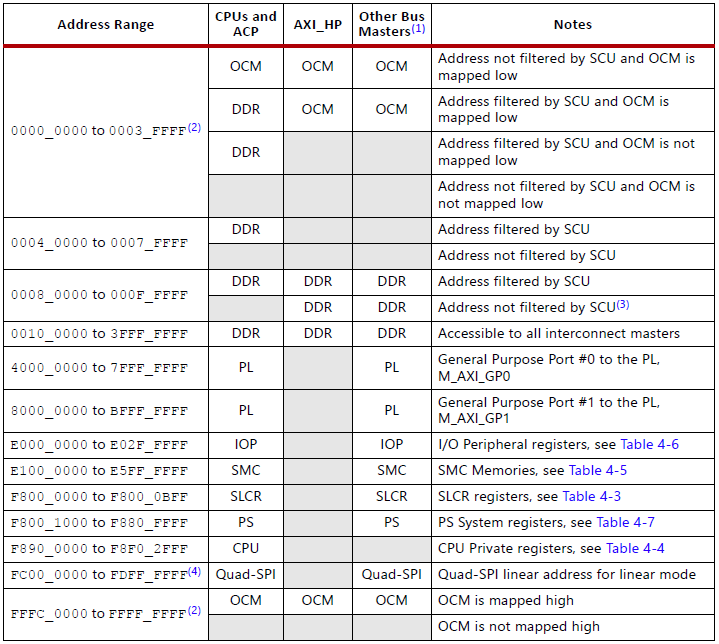
\includegraphics[width=14cm,height=\textheight,keepaspectratio]{images/AddressMapZynq.png}
	\caption[]{Address Map des Zynq}
	\label{fig:AddressMapZynq}
\end{figure}


\section{Floating Point Unit}
FPUs (\textit{Floating Point  Unit}) können je nach Implementation unterschiedliche Funktionen unterstützen.
In den Registern MVFR0 und MVFR (\textit{Media and VFP Feature Register}) lässt sich auslesen welche Funktionen in der Hardware implementiert wurden und genutzt werden können.
Diese Register können aber nicht mit einer einfachen \textit{Memory read} gelesen werden.
Um diese Register oder die anderen speziellen FPU-Register, wie FPSID, FPSCR und PFEXC, lesen zu können, muss die ARM-Instruktion \textit{''VMRS''} verwendet werden.

\subsection{FPU initialisieren}
Damit auf die FPU zugegriffen werden kann, muss der Co-Prozessor 15 erst so konfiguriert werden, dass das System im \textit{secure} und im \textit{non-secure mode} Zugriff auf die FPU hat.
Der CP15 ist ein \textit{''System control coprocessor''}, der neben der FPU auch den Cache und die MPU (Memory Protection Unit) konfiguriert.
Um in ein Register des Co-Prozessors schreiben zu können, muss eine spezielle Instruktion \texttt{''MCR''} verwendet werden, die ein ARM-Register in ein Co-Prozessor-Register speichert.
Da OpenOCD diese Instruktion unterstützt, können die \textit{Access Control Register} direkt mit dem Debugger gesetzt werden.

Das NSACR (\textit{Non-secure Access Control Register}) kontrolliert, ob die FPU auch im \textit{non-secure mode} genutzt werden kann.
Das CPACR (\textit{Coprocessor Access Control Register)} kontrolliert den Zugang zu allen Coprozessoren (CP10 und CP11 sind die FPU).

Zusätzlich muss auch noch das FPEXC EN Bit im FPEXC Register (\textit{Floating-Point Satus and Control Register}) gesetzt werden.
Das FPEXC Register kann aber nicht mit dem Debugger direkt gesetzt werden, da eine spezielle ARM Instruktion dafür verwendet werden muss.
Im Kapitel \textit{''2.4.2 Accessing the FPU registers} des FPU-TRM\cite{bib:FPUTechnicalReferenceManual} sind die Details beschrieben, welche Register genau gesetzt werden müssen.

Mit dem folgenden ARM Code kann die FPU z.B. beim Booten des Kernels initialisiert werden:

\lstset{language=[x86masm]Assembler}
\begin{lstlisting}[frame=single]
; Set bits [11:10] of the NSACR for access to CP10 and CP11 from both Secure and Non-secure states:
MRC p15, 0, r0, c1, c1, 2
ORR r0, r0, #2_11<<10 ; enable fpu/neon
MCR p15, 0, r0, c1, c1, 2
; Set the CPACR for access to CP10 and CP11:
LDR r0, =(0xF << 20)
MCR p15, 0, r0, c1, c0, 2
; Set the FPEXC EN bit to enable the FPU:
MOV r3, #0x40000000
VMSR FPEXC, r3
\end{lstlisting}


\subsection{MVFR lesen mit OpenOCD}
OpenOCD kann zwar direkt die Register der generischen Co-Prozessoren lesen und schreiben, nicht aber die Register der FPU.
Der folgende Ablauf ermöglicht es aber trotzdem, diese Register auszulesen:

\begin{enumerate}
\item OpenOCD starten und für das CLI eine Telnetverbindung zu Port 4444 aufbauen
\item \texttt{reset init}\ \ \ \ \ \textcolor{darkgreen}{// Reset und Initialisierung des ganzen Systems.} 
\item \texttt{arm mcr 15 0 1 1 2 0x0c00}\ \ \ \ \ \textcolor{darkgreen}{// Non-secure access für FPU (NSACR Register).} 
\item \texttt{arm mcr 15 0 1 0 2 0x00f00000}\ \ \ \ \ \textcolor{darkgreen}{// Genereller Zugang für FPU erlauben (CPACR Register).} 
\item \texttt{mww 0x0 0xEEF70A10}\ \ \ \ \ \textcolor{darkgreen}{// Speichert die Instruktion \texttt{''VMRS R0, MVFR0''} in den OCM.}
\item \texttt{mww 0x4 0xEEF61A10}\ \ \ \ \ \textcolor{darkgreen}{// Speichert die Instruktion \texttt{''VMRS R1, MVFR1''} in den OCM.}
\item \texttt{bp 0x8 1 hw}\ \ \ \ \ \textcolor{darkgreen}{// Breakpoint nach der Instruktion (32 Bit Instruktion = 4 Byte)}
\item \texttt{resume 0x0}\ \ \ \ \ \textcolor{darkgreen}{// Führt die Instruktion bei der Adresse 0 aus}
\item \texttt{reg 0}\ \ \ \ \ \textcolor{darkgreen}{// Liest dass Register 0 aus, welches eine Kopie des MVFR0 enthält.}
\item \texttt{reg 1}\ \ \ \ \ \textcolor{darkgreen}{// Liest dass Register 1 aus, welches eine Kopie des MVFR1 enthält.}
\end{enumerate}

Die Inhalte der Register sind:
\begin{itemize}
	\item MVFR0:	0x1011\_0222
	\item MVFR1:	0x0111\_1111
\end{itemize}



\subsection{Unterstützte Features der FPU}
Die Register MVFR0 und MVFR1 enthalten Informationen über die unterstützten Features der FPU.
Auf der Seite B5-36 des ARMv7-A ARM\cite{bib:ARMv7ArchitectureReferenceManual} (\textit{Architecture Reference Manual}) ist beschrieben, wie die unterstützten Features aus den Registern gelesen werden können.

Der Zynq des Zybo unterstützt:
\begin{itemize}
	\item All rounding modes
	\item VFP squarde root operations
	\item VFP divide operations
	\item Full VFP douple-precision v3 (VFPv3)
	\item VFPv3 single-precision
	\item Advanced SIMD register bank: 32 x 64-bit registers
	\item All VFP instructions (\texttt{LDC, STC, MCR,} and \texttt{MRC})
	\item Half-precision floating-point conversion operations (VFP and advanced SIMD)
	\item Single-precision floating-point operations (advanced SIMD)
	\item Integer operations (advanced SIMD)
	\item Load/store operations (advanced SIMD)
	\item Propagation of NaN values
\end{itemize}

Nicht unterstützt wird:
\begin{itemize}
	\item VFP short vectors
	\item VFP exception trapping
\end{itemize}





